% Options for packages loaded elsewhere
\PassOptionsToPackage{unicode}{hyperref}
\PassOptionsToPackage{hyphens}{url}
%
\documentclass[
]{article}
\usepackage{amsmath,amssymb}
\usepackage{iftex}
\ifPDFTeX
  \usepackage[T1]{fontenc}
  \usepackage[utf8]{inputenc}
  \usepackage{textcomp} % provide euro and other symbols
\else % if luatex or xetex
  \usepackage{unicode-math} % this also loads fontspec
  \defaultfontfeatures{Scale=MatchLowercase}
  \defaultfontfeatures[\rmfamily]{Ligatures=TeX,Scale=1}
\fi
\usepackage{lmodern}
\ifPDFTeX\else
  % xetex/luatex font selection
    \setmainfont[]{NanumGothic}
    \setmonofont[]{UnShinmun}
\fi
% Use upquote if available, for straight quotes in verbatim environments
\IfFileExists{upquote.sty}{\usepackage{upquote}}{}
\IfFileExists{microtype.sty}{% use microtype if available
  \usepackage[]{microtype}
  \UseMicrotypeSet[protrusion]{basicmath} % disable protrusion for tt fonts
}{}
\makeatletter
\@ifundefined{KOMAClassName}{% if non-KOMA class
  \IfFileExists{parskip.sty}{%
    \usepackage{parskip}
  }{% else
    \setlength{\parindent}{0pt}
    \setlength{\parskip}{6pt plus 2pt minus 1pt}}
}{% if KOMA class
  \KOMAoptions{parskip=half}}
\makeatother
\usepackage{xcolor}
\usepackage[margin=1in]{geometry}
\usepackage{color}
\usepackage{fancyvrb}
\newcommand{\VerbBar}{|}
\newcommand{\VERB}{\Verb[commandchars=\\\{\}]}
\DefineVerbatimEnvironment{Highlighting}{Verbatim}{commandchars=\\\{\}}
% Add ',fontsize=\small' for more characters per line
\usepackage{framed}
\definecolor{shadecolor}{RGB}{248,248,248}
\newenvironment{Shaded}{\begin{snugshade}}{\end{snugshade}}
\newcommand{\AlertTok}[1]{\textcolor[rgb]{0.94,0.16,0.16}{#1}}
\newcommand{\AnnotationTok}[1]{\textcolor[rgb]{0.56,0.35,0.01}{\textbf{\textit{#1}}}}
\newcommand{\AttributeTok}[1]{\textcolor[rgb]{0.13,0.29,0.53}{#1}}
\newcommand{\BaseNTok}[1]{\textcolor[rgb]{0.00,0.00,0.81}{#1}}
\newcommand{\BuiltInTok}[1]{#1}
\newcommand{\CharTok}[1]{\textcolor[rgb]{0.31,0.60,0.02}{#1}}
\newcommand{\CommentTok}[1]{\textcolor[rgb]{0.56,0.35,0.01}{\textit{#1}}}
\newcommand{\CommentVarTok}[1]{\textcolor[rgb]{0.56,0.35,0.01}{\textbf{\textit{#1}}}}
\newcommand{\ConstantTok}[1]{\textcolor[rgb]{0.56,0.35,0.01}{#1}}
\newcommand{\ControlFlowTok}[1]{\textcolor[rgb]{0.13,0.29,0.53}{\textbf{#1}}}
\newcommand{\DataTypeTok}[1]{\textcolor[rgb]{0.13,0.29,0.53}{#1}}
\newcommand{\DecValTok}[1]{\textcolor[rgb]{0.00,0.00,0.81}{#1}}
\newcommand{\DocumentationTok}[1]{\textcolor[rgb]{0.56,0.35,0.01}{\textbf{\textit{#1}}}}
\newcommand{\ErrorTok}[1]{\textcolor[rgb]{0.64,0.00,0.00}{\textbf{#1}}}
\newcommand{\ExtensionTok}[1]{#1}
\newcommand{\FloatTok}[1]{\textcolor[rgb]{0.00,0.00,0.81}{#1}}
\newcommand{\FunctionTok}[1]{\textcolor[rgb]{0.13,0.29,0.53}{\textbf{#1}}}
\newcommand{\ImportTok}[1]{#1}
\newcommand{\InformationTok}[1]{\textcolor[rgb]{0.56,0.35,0.01}{\textbf{\textit{#1}}}}
\newcommand{\KeywordTok}[1]{\textcolor[rgb]{0.13,0.29,0.53}{\textbf{#1}}}
\newcommand{\NormalTok}[1]{#1}
\newcommand{\OperatorTok}[1]{\textcolor[rgb]{0.81,0.36,0.00}{\textbf{#1}}}
\newcommand{\OtherTok}[1]{\textcolor[rgb]{0.56,0.35,0.01}{#1}}
\newcommand{\PreprocessorTok}[1]{\textcolor[rgb]{0.56,0.35,0.01}{\textit{#1}}}
\newcommand{\RegionMarkerTok}[1]{#1}
\newcommand{\SpecialCharTok}[1]{\textcolor[rgb]{0.81,0.36,0.00}{\textbf{#1}}}
\newcommand{\SpecialStringTok}[1]{\textcolor[rgb]{0.31,0.60,0.02}{#1}}
\newcommand{\StringTok}[1]{\textcolor[rgb]{0.31,0.60,0.02}{#1}}
\newcommand{\VariableTok}[1]{\textcolor[rgb]{0.00,0.00,0.00}{#1}}
\newcommand{\VerbatimStringTok}[1]{\textcolor[rgb]{0.31,0.60,0.02}{#1}}
\newcommand{\WarningTok}[1]{\textcolor[rgb]{0.56,0.35,0.01}{\textbf{\textit{#1}}}}
\usepackage{graphicx}
\makeatletter
\def\maxwidth{\ifdim\Gin@nat@width>\linewidth\linewidth\else\Gin@nat@width\fi}
\def\maxheight{\ifdim\Gin@nat@height>\textheight\textheight\else\Gin@nat@height\fi}
\makeatother
% Scale images if necessary, so that they will not overflow the page
% margins by default, and it is still possible to overwrite the defaults
% using explicit options in \includegraphics[width, height, ...]{}
\setkeys{Gin}{width=\maxwidth,height=\maxheight,keepaspectratio}
% Set default figure placement to htbp
\makeatletter
\def\fps@figure{htbp}
\makeatother
\setlength{\emergencystretch}{3em} % prevent overfull lines
\providecommand{\tightlist}{%
  \setlength{\itemsep}{0pt}\setlength{\parskip}{0pt}}
\setcounter{secnumdepth}{-\maxdimen} % remove section numbering
\usepackage{fvextra}
\fvset{breaklines}
\ifLuaTeX
  \usepackage{selnolig}  % disable illegal ligatures
\fi
\usepackage{bookmark}
\IfFileExists{xurl.sty}{\usepackage{xurl}}{} % add URL line breaks if available
\urlstyle{same}
\hypersetup{
  pdftitle={multivariate\_hw7},
  pdfauthor={Na SeungChan},
  hidelinks,
  pdfcreator={LaTeX via pandoc}}

\title{multivariate\_hw7}
\author{Na SeungChan}
\date{2024-12-10}

\begin{document}
\maketitle

\begin{center}\rule{0.5\linewidth}{0.5pt}\end{center}

\section{Q 6.1}\label{q-6.1}

\begin{Shaded}
\begin{Highlighting}[]
\NormalTok{x1\_c }\OtherTok{\textless{}{-}} \FunctionTok{c}\NormalTok{(}\DecValTok{6}\NormalTok{, }\DecValTok{6}\NormalTok{, }\DecValTok{18}\NormalTok{, }\DecValTok{8}\NormalTok{, }\DecValTok{11}\NormalTok{, }\DecValTok{34}\NormalTok{, }\DecValTok{28}\NormalTok{, }\DecValTok{71}\NormalTok{, }\DecValTok{43}\NormalTok{, }\DecValTok{33}\NormalTok{, }\DecValTok{20}\NormalTok{)}
\NormalTok{x1\_s }\OtherTok{\textless{}{-}} \FunctionTok{c}\NormalTok{(}\DecValTok{25}\NormalTok{, }\DecValTok{28}\NormalTok{, }\DecValTok{36}\NormalTok{, }\DecValTok{35}\NormalTok{, }\DecValTok{15}\NormalTok{, }\DecValTok{44}\NormalTok{, }\DecValTok{42}\NormalTok{, }\DecValTok{54}\NormalTok{, }\DecValTok{34}\NormalTok{, }\DecValTok{29}\NormalTok{, }\DecValTok{39}\NormalTok{)}
\NormalTok{x2\_c }\OtherTok{\textless{}{-}} \FunctionTok{c}\NormalTok{(}\DecValTok{27}\NormalTok{, }\DecValTok{23}\NormalTok{, }\DecValTok{64}\NormalTok{, }\DecValTok{44}\NormalTok{, }\DecValTok{30}\NormalTok{, }\DecValTok{75}\NormalTok{, }\DecValTok{26}\NormalTok{, }\DecValTok{124}\NormalTok{, }\DecValTok{54}\NormalTok{, }\DecValTok{30}\NormalTok{, }\DecValTok{14}\NormalTok{)}
\NormalTok{x2\_s }\OtherTok{\textless{}{-}} \FunctionTok{c}\NormalTok{(}\DecValTok{15}\NormalTok{, }\DecValTok{13}\NormalTok{, }\DecValTok{22}\NormalTok{, }\DecValTok{29}\NormalTok{, }\DecValTok{31}\NormalTok{, }\DecValTok{64}\NormalTok{, }\DecValTok{30}\NormalTok{, }\DecValTok{64}\NormalTok{, }\DecValTok{56}\NormalTok{, }\DecValTok{20}\NormalTok{, }\DecValTok{21}\NormalTok{)}

\NormalTok{df }\OtherTok{\textless{}{-}} \FunctionTok{tibble}\NormalTok{(x1\_c, x1\_s, x2\_c, x2\_s)}
\end{Highlighting}
\end{Shaded}

\begin{Shaded}
\begin{Highlighting}[]
\NormalTok{diff\_df }\OtherTok{\textless{}{-}}\NormalTok{ df }\SpecialCharTok{\%\textgreater{}\%} 
  \FunctionTok{transmute}\NormalTok{(}\AttributeTok{diff\_x1 =}\NormalTok{ x1\_c }\SpecialCharTok{{-}}\NormalTok{ x1\_s, }\AttributeTok{diff\_x2 =}\NormalTok{ x2\_c }\SpecialCharTok{{-}}\NormalTok{ x2\_s)}
\end{Highlighting}
\end{Shaded}

\begin{Shaded}
\begin{Highlighting}[]
\NormalTok{mean\_df }\OtherTok{\textless{}{-}} \FunctionTok{colMeans}\NormalTok{(diff\_df)}
\NormalTok{mean\_df}
\end{Highlighting}
\end{Shaded}

\begin{verbatim}
##   diff_x1   diff_x2 
## -9.363636 13.272727
\end{verbatim}

\begin{Shaded}
\begin{Highlighting}[]
\NormalTok{var\_df }\OtherTok{\textless{}{-}} \FunctionTok{cov}\NormalTok{(diff\_df)}
\NormalTok{var\_df}
\end{Highlighting}
\end{Shaded}

\begin{verbatim}
##           diff_x1   diff_x2
## diff_x1 199.25455  88.30909
## diff_x2  88.30909 418.61818
\end{verbatim}

교재의 \(S_d\)와 데이터 매트릭스를 직접 입력해 계산한 \(S_d\)의 값이
약간 다르다. 문제풀이에서는 데이터 매트릭스를 직접 입력해 계산한 값을
활용해 계산한다.

\begin{Shaded}
\begin{Highlighting}[]
\FunctionTok{sqrt}\NormalTok{(}\FunctionTok{eigen}\NormalTok{(var\_df)}\SpecialCharTok{$}\NormalTok{values)}
\end{Highlighting}
\end{Shaded}

\begin{verbatim}
## [1] 21.20732 12.96620
\end{verbatim}

\begin{Shaded}
\begin{Highlighting}[]
\FunctionTok{eigen}\NormalTok{(var\_df)}\SpecialCharTok{$}\NormalTok{vectors}
\end{Highlighting}
\end{Shaded}

\begin{verbatim}
##           [,1]       [,2]
## [1,] 0.3324812 -0.9431099
## [2,] 0.9431099  0.3324812
\end{verbatim}

\section{Q 6.2}\label{q-6.2}

\begin{Shaded}
\begin{Highlighting}[]
\NormalTok{crit\_v1 }\OtherTok{\textless{}{-}} \FunctionTok{sqrt}\NormalTok{(var\_df[}\DecValTok{1}\NormalTok{]}\SpecialCharTok{/}\DecValTok{11}\NormalTok{)}\SpecialCharTok{*}\FunctionTok{qt}\NormalTok{(}\DecValTok{1}\SpecialCharTok{/}\DecValTok{80}\NormalTok{, }\AttributeTok{df =} \DecValTok{10}\NormalTok{, }\AttributeTok{lower.tail =} \ConstantTok{FALSE}\NormalTok{)}
\NormalTok{BCI\_V1 }\OtherTok{\textless{}{-}} \FunctionTok{c}\NormalTok{(mean\_df[}\DecValTok{1}\NormalTok{] }\SpecialCharTok{{-}}\NormalTok{ crit\_v1, mean\_df[}\DecValTok{1}\NormalTok{] }\SpecialCharTok{+}\NormalTok{ crit\_v1)}
\NormalTok{crit\_v2 }\OtherTok{\textless{}{-}} \FunctionTok{sqrt}\NormalTok{(var\_df[}\DecValTok{4}\NormalTok{]}\SpecialCharTok{/}\DecValTok{11}\NormalTok{)}\SpecialCharTok{*}\FunctionTok{qt}\NormalTok{(}\DecValTok{1}\SpecialCharTok{/}\DecValTok{80}\NormalTok{, }\AttributeTok{df =} \DecValTok{10}\NormalTok{, }\AttributeTok{lower.tail =} \ConstantTok{FALSE}\NormalTok{)}
\NormalTok{BCI\_V2 }\OtherTok{\textless{}{-}} \FunctionTok{c}\NormalTok{(mean\_df[}\DecValTok{2}\NormalTok{] }\SpecialCharTok{{-}}\NormalTok{ crit\_v2, mean\_df[}\DecValTok{2}\NormalTok{] }\SpecialCharTok{+}\NormalTok{ crit\_v2)}
\end{Highlighting}
\end{Shaded}

\begin{Shaded}
\begin{Highlighting}[]
\NormalTok{BCI\_V1}
\end{Highlighting}
\end{Shaded}

\begin{verbatim}
##    diff_x1    diff_x1 
## -20.573107   1.845835
\end{verbatim}

\begin{Shaded}
\begin{Highlighting}[]
\NormalTok{BCI\_V2}
\end{Highlighting}
\end{Shaded}

\begin{verbatim}
##   diff_x2   diff_x2 
## -2.974903 29.520358
\end{verbatim}

example 6.1의 동시 신뢰구간은 \texttt{diff\_x1}의 경우 (-22.46, 3.74),
\texttt{diff\_x2}의 경우 (-5.71, 32.25)이다. 여기서 구한 본페르니
신뢰구간이 동시 신뢰구간에 비해 V1과 V2 모두 upper bound가 작고 lower
bound가 커서 신뢰구간이 더 좁은 것을 볼 수 있다.

\section{Q 6.3}\label{q-6.3}

\begin{Shaded}
\begin{Highlighting}[]
\NormalTok{diff\_q3 }\OtherTok{\textless{}{-}}\NormalTok{ diff\_df }\SpecialCharTok{\%\textgreater{}\%} \FunctionTok{slice}\NormalTok{(}\SpecialCharTok{{-}}\DecValTok{8}\NormalTok{)}
\NormalTok{xbar }\OtherTok{\textless{}{-}} \FunctionTok{colMeans}\NormalTok{(diff\_q3)}
\NormalTok{Smtx }\OtherTok{\textless{}{-}} \FunctionTok{cov}\NormalTok{(diff\_q3)}
\end{Highlighting}
\end{Shaded}

위와 같이 이상치를 제거한 데이터프레임을 구하였고, 평균벡터와 분산행렬을
구하였다.

동시 신뢰구간

\begin{Shaded}
\begin{Highlighting}[]
\NormalTok{crit }\OtherTok{\textless{}{-}} \FunctionTok{sqrt}\NormalTok{(}\FunctionTok{qf}\NormalTok{(}\FloatTok{0.05}\NormalTok{, }\DecValTok{2}\NormalTok{, }\DecValTok{8}\NormalTok{, }\AttributeTok{lower.tail =} \ConstantTok{FALSE}\NormalTok{) }\SpecialCharTok{*}\NormalTok{ (}\DecValTok{2}\SpecialCharTok{*}\DecValTok{9}\SpecialCharTok{/}\DecValTok{8}\NormalTok{))}
\NormalTok{SCI\_V1 }\OtherTok{\textless{}{-}} \FunctionTok{c}\NormalTok{(xbar[}\DecValTok{1}\NormalTok{] }\SpecialCharTok{{-}}\NormalTok{ crit}\SpecialCharTok{*}\FunctionTok{sqrt}\NormalTok{(Smtx[}\DecValTok{1}\NormalTok{]}\SpecialCharTok{/}\DecValTok{10}\NormalTok{), xbar[}\DecValTok{1}\NormalTok{] }\SpecialCharTok{+}\NormalTok{ crit}\SpecialCharTok{*}\FunctionTok{sqrt}\NormalTok{(Smtx[}\DecValTok{1}\NormalTok{]}\SpecialCharTok{/}\DecValTok{10}\NormalTok{))}
\NormalTok{SCI\_V2 }\OtherTok{\textless{}{-}} \FunctionTok{c}\NormalTok{(xbar[}\DecValTok{2}\NormalTok{] }\SpecialCharTok{{-}}\NormalTok{ crit}\SpecialCharTok{*}\FunctionTok{sqrt}\NormalTok{(Smtx[}\DecValTok{4}\NormalTok{]}\SpecialCharTok{/}\DecValTok{10}\NormalTok{), xbar[}\DecValTok{2}\NormalTok{] }\SpecialCharTok{+}\NormalTok{ crit}\SpecialCharTok{*}\FunctionTok{sqrt}\NormalTok{(Smtx[}\DecValTok{4}\NormalTok{]}\SpecialCharTok{/}\DecValTok{10}\NormalTok{))}
\end{Highlighting}
\end{Shaded}

\begin{Shaded}
\begin{Highlighting}[]
\FunctionTok{eigen}\NormalTok{(Smtx)}
\end{Highlighting}
\end{Shaded}

\begin{verbatim}
## eigen() decomposition
## $values
## [1] 228.2318 106.4793
## 
## $vectors
##            [,1]       [,2]
## [1,] -0.4960999 -0.8682654
## [2,]  0.8682654 -0.4960999
\end{verbatim}

본페르니 신뢰구간

\begin{Shaded}
\begin{Highlighting}[]
\NormalTok{crit\_v1 }\OtherTok{\textless{}{-}} \FunctionTok{sqrt}\NormalTok{(Smtx[}\DecValTok{1}\NormalTok{]}\SpecialCharTok{/}\DecValTok{10}\NormalTok{)}\SpecialCharTok{*}\FunctionTok{qt}\NormalTok{(}\DecValTok{1}\SpecialCharTok{/}\DecValTok{80}\NormalTok{, }\AttributeTok{df =} \DecValTok{9}\NormalTok{, }\AttributeTok{lower.tail =} \ConstantTok{FALSE}\NormalTok{)}
\NormalTok{BCI\_V1 }\OtherTok{\textless{}{-}} \FunctionTok{c}\NormalTok{(xbar[}\DecValTok{1}\NormalTok{] }\SpecialCharTok{{-}}\NormalTok{ crit\_v1, xbar[}\DecValTok{1}\NormalTok{] }\SpecialCharTok{+}\NormalTok{ crit\_v1)}
\NormalTok{crit\_v2 }\OtherTok{\textless{}{-}} \FunctionTok{sqrt}\NormalTok{(Smtx[}\DecValTok{4}\NormalTok{]}\SpecialCharTok{/}\DecValTok{10}\NormalTok{)}\SpecialCharTok{*}\FunctionTok{qt}\NormalTok{(}\DecValTok{1}\SpecialCharTok{/}\DecValTok{80}\NormalTok{, }\AttributeTok{df =} \DecValTok{9}\NormalTok{, }\AttributeTok{lower.tail =} \ConstantTok{FALSE}\NormalTok{)}
\NormalTok{BCI\_V2 }\OtherTok{\textless{}{-}} \FunctionTok{c}\NormalTok{(xbar[}\DecValTok{2}\NormalTok{] }\SpecialCharTok{{-}}\NormalTok{ crit\_v2, xbar[}\DecValTok{2}\NormalTok{] }\SpecialCharTok{+}\NormalTok{ crit\_v2)}
\end{Highlighting}
\end{Shaded}

\begin{Shaded}
\begin{Highlighting}[]
\NormalTok{SCI\_V1}
\end{Highlighting}
\end{Shaded}

\begin{verbatim}
##     diff_x1     diff_x1 
## -23.7000163  -0.2999837
\end{verbatim}

\begin{Shaded}
\begin{Highlighting}[]
\NormalTok{BCI\_V1}
\end{Highlighting}
\end{Shaded}

\begin{verbatim}
##    diff_x1    diff_x1 
## -21.917997  -2.082003
\end{verbatim}

\begin{Shaded}
\begin{Highlighting}[]
\NormalTok{SCI\_V2}
\end{Highlighting}
\end{Shaded}

\begin{verbatim}
##   diff_x2   diff_x2 
## -5.503711 22.703711
\end{verbatim}

\begin{Shaded}
\begin{Highlighting}[]
\NormalTok{BCI\_V2}
\end{Highlighting}
\end{Shaded}

\begin{verbatim}
##   diff_x2   diff_x2 
## -3.355587 20.555587
\end{verbatim}

동시 신뢰구간 SCI\_V1, SCI\_V2가 (0,0) point를 포함하지 않으므로
이상치를 기각한 경우에도 example 6.1과 같이 귀무가설을 기각하게 된다.
이상치 유무와 관계없이 귀무가설을 기각하지만, 이 경우에는 동시
신뢰구간이 0을 포함하는 상황 자체가 존재하지 않아 example 6.1에 비해
유의수준이 높을 것이다.

\section{Q 6.4}\label{q-6.4}

\begin{Shaded}
\begin{Highlighting}[]
\NormalTok{tdf }\OtherTok{\textless{}{-}} \FunctionTok{log}\NormalTok{(df) }\SpecialCharTok{\%\textgreater{}\%} \FunctionTok{transmute}\NormalTok{(}\AttributeTok{dx1 =}\NormalTok{ x1\_c }\SpecialCharTok{{-}}\NormalTok{ x1\_s, }\AttributeTok{dx2 =}\NormalTok{ x2\_c }\SpecialCharTok{{-}}\NormalTok{ x2\_s)}
\NormalTok{tdf}
\end{Highlighting}
\end{Shaded}

\begin{verbatim}
## # A tibble: 11 x 2
##       dx1     dx2
##     <dbl>   <dbl>
##  1 -1.43   0.588 
##  2 -1.54   0.571 
##  3 -0.693  1.07  
##  4 -1.48   0.417 
##  5 -0.310 -0.0328
##  6 -0.258  0.159 
##  7 -0.405 -0.143 
##  8  0.274  0.661 
##  9  0.235 -0.0364
## 10  0.129  0.405 
## 11 -0.668 -0.405
\end{verbatim}

로그 변환된 데이터프레임을 계산하였다.

\subsection{(a)}\label{a}

\begin{Shaded}
\begin{Highlighting}[]
\NormalTok{xbar }\OtherTok{\textless{}{-}} \FunctionTok{colMeans}\NormalTok{(tdf)}
\NormalTok{Smtx }\OtherTok{\textless{}{-}} \FunctionTok{cov}\NormalTok{(tdf)}
\end{Highlighting}
\end{Shaded}

\subsubsection{Hotelling's T\^{}2 test}\label{hotellings-t2-test}

\begin{Shaded}
\begin{Highlighting}[]
\NormalTok{test\_statistics }\OtherTok{\textless{}{-}} \DecValTok{11} \SpecialCharTok{*} \FunctionTok{t}\NormalTok{(xbar) }\SpecialCharTok{\%*\%} \FunctionTok{solve}\NormalTok{(Smtx) }\SpecialCharTok{\%*\%}\NormalTok{ (xbar)}
\NormalTok{critical\_value }\OtherTok{\textless{}{-}} \FunctionTok{qf}\NormalTok{(}\FloatTok{0.05}\NormalTok{, }\DecValTok{2}\NormalTok{, }\DecValTok{9}\NormalTok{, }\AttributeTok{lower.tail =} \ConstantTok{FALSE}\NormalTok{) }\SpecialCharTok{*}\NormalTok{ (}\DecValTok{2}\SpecialCharTok{*}\DecValTok{10}\SpecialCharTok{/}\DecValTok{9}\NormalTok{)}
\NormalTok{test\_statistics}
\end{Highlighting}
\end{Shaded}

\begin{verbatim}
##          [,1]
## [1,] 10.21541
\end{verbatim}

\begin{Shaded}
\begin{Highlighting}[]
\NormalTok{critical\_value}
\end{Highlighting}
\end{Shaded}

\begin{verbatim}
## [1] 9.458877
\end{verbatim}

\begin{Shaded}
\begin{Highlighting}[]
\NormalTok{test\_statistics }\SpecialCharTok{\textgreater{}}\NormalTok{ critical\_value}
\end{Highlighting}
\end{Shaded}

\begin{verbatim}
##      [,1]
## [1,] TRUE
\end{verbatim}

검정 결과 차이가 있다는 귀무가설을 기각하게 된다.

\subsection{(b)}\label{b}

\begin{Shaded}
\begin{Highlighting}[]
\NormalTok{crit\_v1 }\OtherTok{\textless{}{-}} \FunctionTok{sqrt}\NormalTok{(Smtx[}\DecValTok{1}\NormalTok{]}\SpecialCharTok{/}\DecValTok{11}\NormalTok{)}\SpecialCharTok{*}\FunctionTok{qt}\NormalTok{(}\DecValTok{1}\SpecialCharTok{/}\DecValTok{80}\NormalTok{, }\AttributeTok{df =} \DecValTok{10}\NormalTok{, }\AttributeTok{lower.tail =} \ConstantTok{FALSE}\NormalTok{)}
\NormalTok{BCI\_V1 }\OtherTok{\textless{}{-}} \FunctionTok{c}\NormalTok{(xbar[}\DecValTok{1}\NormalTok{] }\SpecialCharTok{{-}}\NormalTok{ crit\_v1, xbar[}\DecValTok{1}\NormalTok{] }\SpecialCharTok{+}\NormalTok{ crit\_v1)}
\NormalTok{crit\_v2 }\OtherTok{\textless{}{-}} \FunctionTok{sqrt}\NormalTok{(Smtx[}\DecValTok{4}\NormalTok{]}\SpecialCharTok{/}\DecValTok{11}\NormalTok{)}\SpecialCharTok{*}\FunctionTok{qt}\NormalTok{(}\DecValTok{1}\SpecialCharTok{/}\DecValTok{80}\NormalTok{, }\AttributeTok{df =} \DecValTok{10}\NormalTok{, }\AttributeTok{lower.tail =} \ConstantTok{FALSE}\NormalTok{)}
\NormalTok{BCI\_V2 }\OtherTok{\textless{}{-}} \FunctionTok{c}\NormalTok{(xbar[}\DecValTok{2}\NormalTok{] }\SpecialCharTok{{-}}\NormalTok{ crit\_v2, xbar[}\DecValTok{2}\NormalTok{] }\SpecialCharTok{+}\NormalTok{ crit\_v2)}
\end{Highlighting}
\end{Shaded}

\begin{Shaded}
\begin{Highlighting}[]
\NormalTok{BCI\_V1}
\end{Highlighting}
\end{Shaded}

\begin{verbatim}
##         dx1         dx1 
## -1.09448795 -0.02190232
\end{verbatim}

\begin{Shaded}
\begin{Highlighting}[]
\NormalTok{BCI\_V2}
\end{Highlighting}
\end{Shaded}

\begin{verbatim}
##         dx2         dx2 
## -0.04498455  0.63604112
\end{verbatim}

본페르니 신뢰구간은 위와 같다.

\subsection{(c)}\label{c}

\begin{Shaded}
\begin{Highlighting}[]
\FunctionTok{qqnorm}\NormalTok{(tdf}\SpecialCharTok{$}\NormalTok{dx1); }\FunctionTok{qqline}\NormalTok{(tdf}\SpecialCharTok{$}\NormalTok{dx1)}
\end{Highlighting}
\end{Shaded}

\begin{center}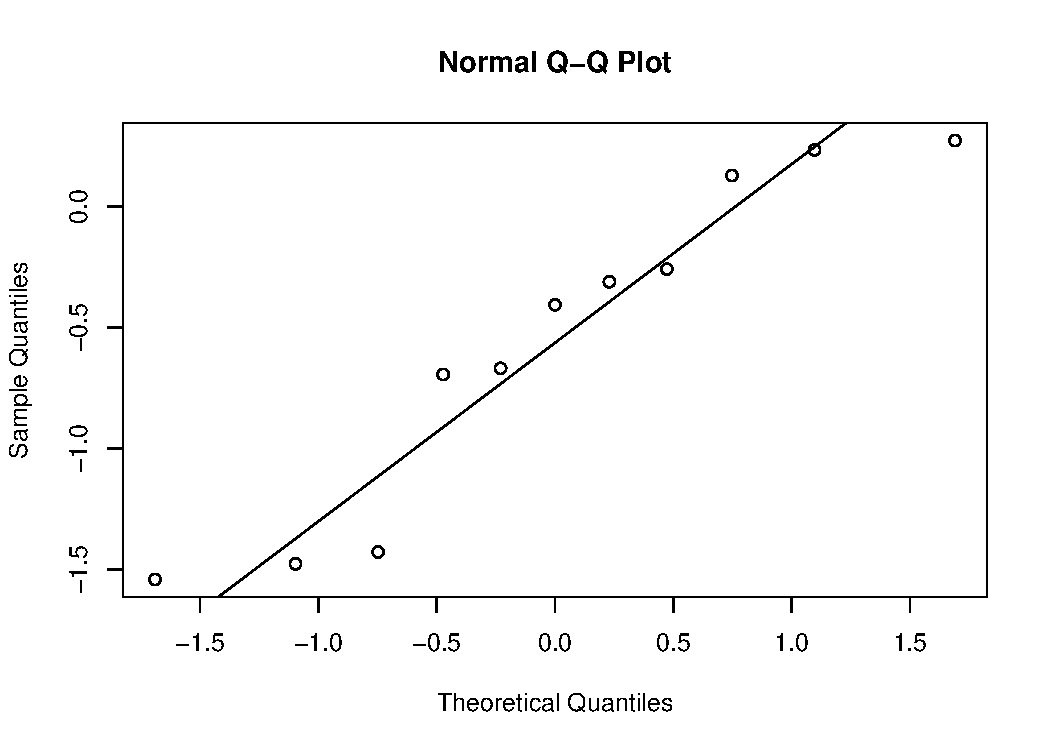
\includegraphics[width=0.8\linewidth]{multi_hw7_files/figure-latex/unnamed-chunk-17-1} \end{center}

\begin{Shaded}
\begin{Highlighting}[]
\FunctionTok{qqnorm}\NormalTok{(tdf}\SpecialCharTok{$}\NormalTok{dx2); }\FunctionTok{qqline}\NormalTok{(tdf}\SpecialCharTok{$}\NormalTok{dx2)}
\end{Highlighting}
\end{Shaded}

\begin{center}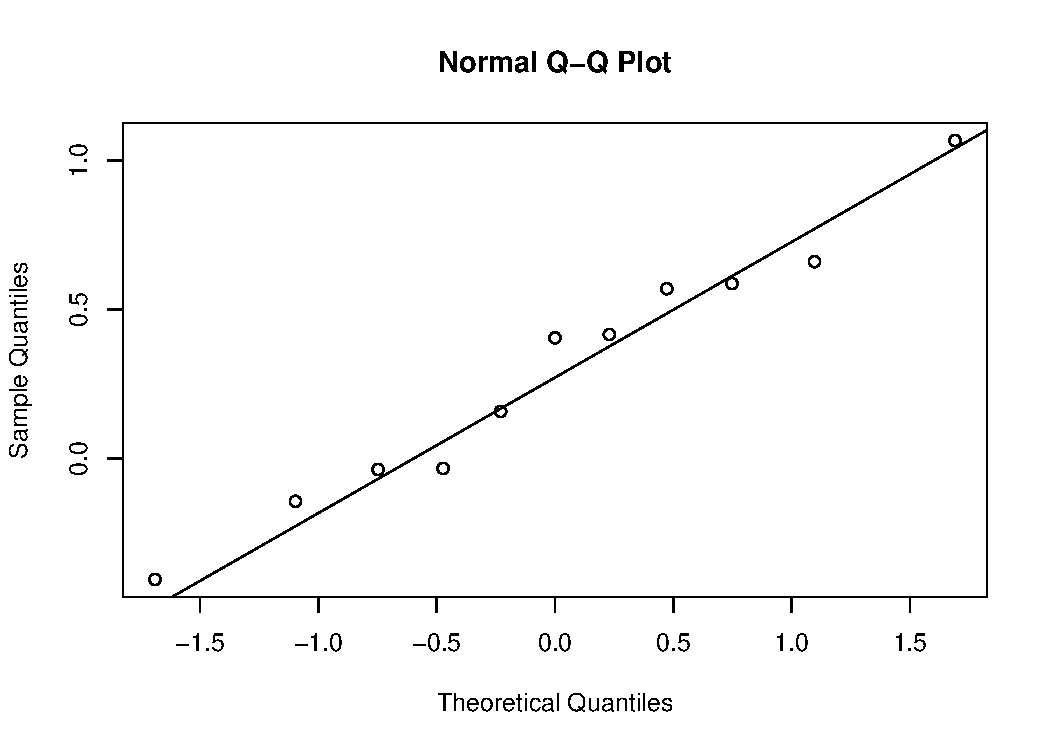
\includegraphics[width=0.8\linewidth]{multi_hw7_files/figure-latex/unnamed-chunk-17-2} \end{center}

marginally normal이라고 볼 수도 있을 것 같다.

\begin{Shaded}
\begin{Highlighting}[]
\NormalTok{Xc }\OtherTok{\textless{}{-}} \FunctionTok{t}\NormalTok{(}\FunctionTok{t}\NormalTok{(tdf) }\SpecialCharTok{{-}}\NormalTok{ xbar)}
\NormalTok{Mdist }\OtherTok{\textless{}{-}} \FunctionTok{sqrt}\NormalTok{( }\FunctionTok{diag}\NormalTok{( Xc }\SpecialCharTok{\%*\%} \FunctionTok{solve}\NormalTok{(Smtx) }\SpecialCharTok{\%*\%} \FunctionTok{t}\NormalTok{(Xc) ) ) }
\FunctionTok{qqplot}\NormalTok{( }\FunctionTok{qchisq}\NormalTok{(}\FunctionTok{ppoints}\NormalTok{(}\DecValTok{11}\NormalTok{), }\AttributeTok{df =} \DecValTok{3}\NormalTok{), Mdist}\SpecialCharTok{\^{}}\DecValTok{2}\NormalTok{)}
\end{Highlighting}
\end{Shaded}

\begin{center}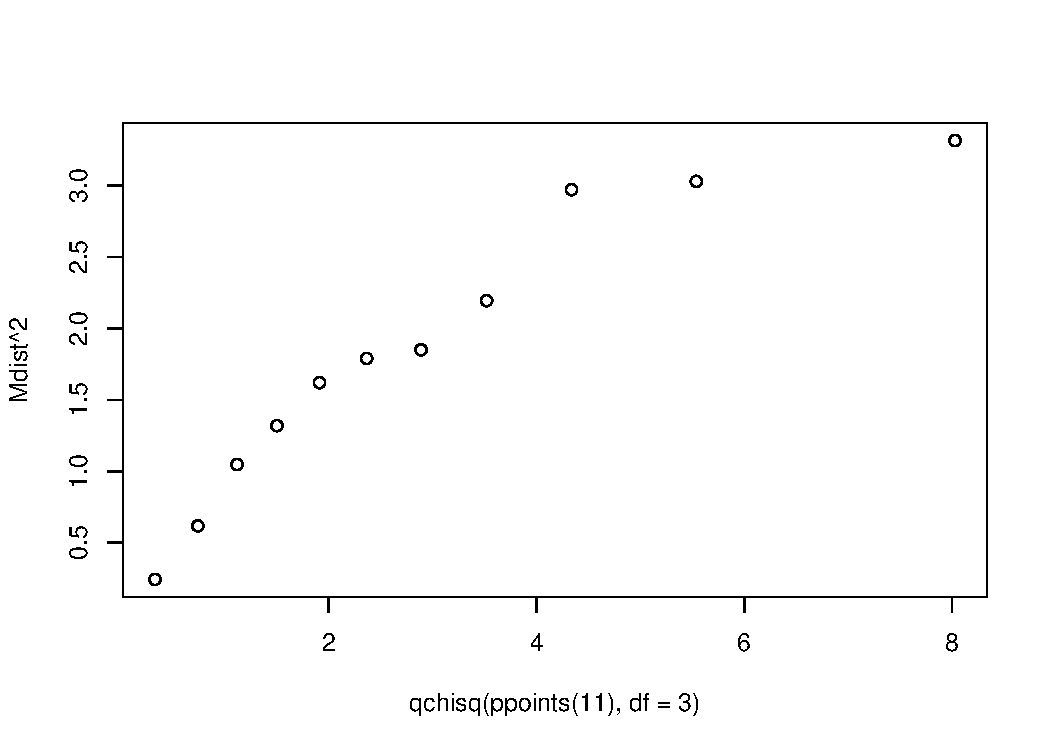
\includegraphics[width=0.8\linewidth]{multi_hw7_files/figure-latex/unnamed-chunk-18-1} \end{center}

n = 11은\ldots{} 정규성 여부를 판단하기 어렵지만, 직선을 따른다고 말하기
어려워 보인다. 즉 joint normal이라고 말하기 어렵다.

\section{Q 6.5}\label{q-6.5}

\begin{Shaded}
\begin{Highlighting}[]
\NormalTok{xbar }\OtherTok{\textless{}{-}} \FunctionTok{c}\NormalTok{(}\FloatTok{46.1}\NormalTok{, }\FloatTok{57.3}\NormalTok{, }\FloatTok{50.4}\NormalTok{)}
\NormalTok{Smtx }\OtherTok{\textless{}{-}} \FunctionTok{matrix}\NormalTok{(}\FunctionTok{c}\NormalTok{(}\FloatTok{101.3}\NormalTok{, }\FloatTok{63.0}\NormalTok{, }\FloatTok{71.0}\NormalTok{, }\FloatTok{63.0}\NormalTok{, }\FloatTok{80.2}\NormalTok{, }\FloatTok{55.6}\NormalTok{, }\FloatTok{71.0}\NormalTok{, }\FloatTok{55.6}\NormalTok{, }\FloatTok{97.4}\NormalTok{), }\AttributeTok{nrow=}\DecValTok{3}\NormalTok{)}
\NormalTok{n }\OtherTok{\textless{}{-}} \DecValTok{40}
\NormalTok{Cmtx }\OtherTok{\textless{}{-}} \FunctionTok{matrix}\NormalTok{(}\FunctionTok{c}\NormalTok{(}\DecValTok{1}\NormalTok{, }\DecValTok{0}\NormalTok{, }\SpecialCharTok{{-}}\DecValTok{1}\NormalTok{, }\DecValTok{1}\NormalTok{, }\DecValTok{0}\NormalTok{, }\SpecialCharTok{{-}}\DecValTok{1}\NormalTok{), }\AttributeTok{nrow =} \DecValTok{2}\NormalTok{)}
\end{Highlighting}
\end{Shaded}

\subsection{(a)}\label{a-1}

\begin{Shaded}
\begin{Highlighting}[]
\NormalTok{test\_statistics }\OtherTok{\textless{}{-}}\NormalTok{ n }\SpecialCharTok{*} \FunctionTok{t}\NormalTok{(Cmtx }\SpecialCharTok{\%*\%}\NormalTok{ xbar) }\SpecialCharTok{\%*\%} \FunctionTok{solve}\NormalTok{(Cmtx }\SpecialCharTok{\%*\%}\NormalTok{ Smtx }\SpecialCharTok{\%*\%} \FunctionTok{t}\NormalTok{(Cmtx)) }\SpecialCharTok{\%*\%}\NormalTok{ (Cmtx }\SpecialCharTok{\%*\%}\NormalTok{ xbar)}
\NormalTok{critical\_value }\OtherTok{\textless{}{-}} \FunctionTok{qf}\NormalTok{(}\FloatTok{0.05}\NormalTok{, }\DecValTok{2}\NormalTok{, }\DecValTok{38}\NormalTok{, }\AttributeTok{lower.tail =} \ConstantTok{FALSE}\NormalTok{) }\SpecialCharTok{*}\NormalTok{ (}\DecValTok{2}\SpecialCharTok{*}\DecValTok{39}\SpecialCharTok{/}\DecValTok{38}\NormalTok{)}
\NormalTok{test\_statistics }\SpecialCharTok{\textgreater{}}\NormalTok{ critical\_value}
\end{Highlighting}
\end{Shaded}

\begin{verbatim}
##      [,1]
## [1,] TRUE
\end{verbatim}

가설 검정 결과 귀무가설을 기각한다. 즉 유의수준 0.05에서 평균이 다르다고
볼 만한 충분한 증거가 있다.

\subsection{(b)}\label{b-1}

\begin{Shaded}
\begin{Highlighting}[]
\CommentTok{\#(mu1 vs. mu3)}
\NormalTok{xbar[}\DecValTok{1}\NormalTok{] }\SpecialCharTok{{-}}\NormalTok{ xbar[}\DecValTok{2}\NormalTok{]}
\end{Highlighting}
\end{Shaded}

\begin{verbatim}
## [1] -11.2
\end{verbatim}

\begin{Shaded}
\begin{Highlighting}[]
\FunctionTok{sqrt}\NormalTok{(critical\_value }\SpecialCharTok{*}\NormalTok{ Smtx[}\DecValTok{1}\NormalTok{] }\SpecialCharTok{/} \DecValTok{40}\NormalTok{)}
\end{Highlighting}
\end{Shaded}

\begin{verbatim}
## [1] 4.107007
\end{verbatim}

\section{Q 6.6}\label{q-6.6}

\begin{Shaded}
\begin{Highlighting}[]
\FunctionTok{qf}\NormalTok{(}\FloatTok{0.01}\NormalTok{, }\DecValTok{2}\NormalTok{, }\DecValTok{4}\NormalTok{, }\AttributeTok{lower.tail =} \ConstantTok{FALSE}\NormalTok{)}\SpecialCharTok{*}\NormalTok{(}\DecValTok{2}\SpecialCharTok{*}\DecValTok{5}\SpecialCharTok{/}\DecValTok{4}\NormalTok{)}
\end{Highlighting}
\end{Shaded}

\begin{verbatim}
## [1] 45
\end{verbatim}

\begin{Shaded}
\begin{Highlighting}[]
\FunctionTok{sqrt}\NormalTok{(}\DecValTok{45}\SpecialCharTok{*}\DecValTok{7}\SpecialCharTok{/}\DecValTok{12}\NormalTok{)}\SpecialCharTok{*}\FunctionTok{sqrt}\NormalTok{(}\DecValTok{8}\SpecialCharTok{/}\DecValTok{5}\NormalTok{)}
\end{Highlighting}
\end{Shaded}

\begin{verbatim}
## [1] 6.480741
\end{verbatim}

\begin{Shaded}
\begin{Highlighting}[]
\FunctionTok{sqrt}\NormalTok{(}\DecValTok{45}\SpecialCharTok{*}\DecValTok{7}\SpecialCharTok{/}\DecValTok{12}\NormalTok{)}\SpecialCharTok{*}\FunctionTok{sqrt}\NormalTok{(}\DecValTok{2}\NormalTok{)}
\end{Highlighting}
\end{Shaded}

\begin{verbatim}
## [1] 7.245688
\end{verbatim}

\section{Q 6.7}\label{q-6.7}

\begin{Shaded}
\begin{Highlighting}[]
\NormalTok{n1 }\OtherTok{\textless{}{-}} \DecValTok{45}
\NormalTok{n2 }\OtherTok{\textless{}{-}} \DecValTok{55}
\NormalTok{xb1 }\OtherTok{\textless{}{-}} \FunctionTok{c}\NormalTok{(}\FloatTok{204.4}\NormalTok{, }\FloatTok{556.6}\NormalTok{)}
\NormalTok{xb2 }\OtherTok{\textless{}{-}} \FunctionTok{c}\NormalTok{(}\FloatTok{130.0}\NormalTok{, }\FloatTok{355.0}\NormalTok{)}
\NormalTok{Sm1 }\OtherTok{\textless{}{-}} \FunctionTok{matrix}\NormalTok{(}\FunctionTok{c}\NormalTok{(}\FloatTok{13825.3}\NormalTok{, }\FloatTok{23823.4}\NormalTok{, }\FloatTok{23823.4}\NormalTok{, }\FloatTok{73107.4}\NormalTok{), }\AttributeTok{nrow =} \DecValTok{2}\NormalTok{)}
\NormalTok{Sm2 }\OtherTok{\textless{}{-}} \FunctionTok{matrix}\NormalTok{(}\FunctionTok{c}\NormalTok{(}\FloatTok{8632.0}\NormalTok{, }\FloatTok{19616.7}\NormalTok{, }\FloatTok{19616.7}\NormalTok{, }\FloatTok{55964.5}\NormalTok{), }\AttributeTok{nrow =} \DecValTok{2}\NormalTok{)}
\NormalTok{Sp }\OtherTok{\textless{}{-}}\NormalTok{ ((n1}\DecValTok{{-}1}\NormalTok{)}\SpecialCharTok{*}\NormalTok{Sm1 }\SpecialCharTok{+}\NormalTok{ (n2}\DecValTok{{-}1}\NormalTok{)}\SpecialCharTok{*}\NormalTok{Sm2)}\SpecialCharTok{/}\NormalTok{(n1 }\SpecialCharTok{+}\NormalTok{ n2 }\SpecialCharTok{{-}} \DecValTok{2}\NormalTok{)}
\end{Highlighting}
\end{Shaded}

\begin{Shaded}
\begin{Highlighting}[]
\NormalTok{critical\_value }\OtherTok{\textless{}{-}} \FunctionTok{qf}\NormalTok{(}\FloatTok{0.05}\NormalTok{, }\DecValTok{2}\NormalTok{, }\DecValTok{97}\NormalTok{, }\AttributeTok{lower.tail =} \ConstantTok{FALSE}\NormalTok{) }\SpecialCharTok{*}\NormalTok{ (}\DecValTok{98}\SpecialCharTok{*}\DecValTok{2}\SpecialCharTok{/}\DecValTok{97}\NormalTok{)}
\NormalTok{test\_statistics }\OtherTok{\textless{}{-}} \FunctionTok{t}\NormalTok{(xb1 }\SpecialCharTok{{-}}\NormalTok{ xb2) }\SpecialCharTok{\%*\%} \FunctionTok{solve}\NormalTok{((}\DecValTok{1}\SpecialCharTok{/}\NormalTok{n1 }\SpecialCharTok{+} \DecValTok{1}\SpecialCharTok{/}\NormalTok{n2)}\SpecialCharTok{*}\NormalTok{Sp) }\SpecialCharTok{\%*\%}\NormalTok{ (xb1 }\SpecialCharTok{{-}}\NormalTok{ xb2)}
\end{Highlighting}
\end{Shaded}

\begin{Shaded}
\begin{Highlighting}[]
\NormalTok{critical\_value}
\end{Highlighting}
\end{Shaded}

\begin{verbatim}
## [1] 6.244089
\end{verbatim}

\begin{Shaded}
\begin{Highlighting}[]
\NormalTok{test\_statistics}
\end{Highlighting}
\end{Shaded}

\begin{verbatim}
##          [,1]
## [1,] 16.06622
\end{verbatim}

\begin{Shaded}
\begin{Highlighting}[]
\FunctionTok{solve}\NormalTok{(Sp) }\SpecialCharTok{\%*\%}\NormalTok{ (xb1 }\SpecialCharTok{{-}}\NormalTok{ xb2)}
\end{Highlighting}
\end{Shaded}

\begin{verbatim}
##            [,1]
## [1,] 0.00170252
## [2,] 0.00259163
\end{verbatim}

\section{Q 6.13}\label{q-6.13}

\end{document}
